\begin{figure}[t]\centering
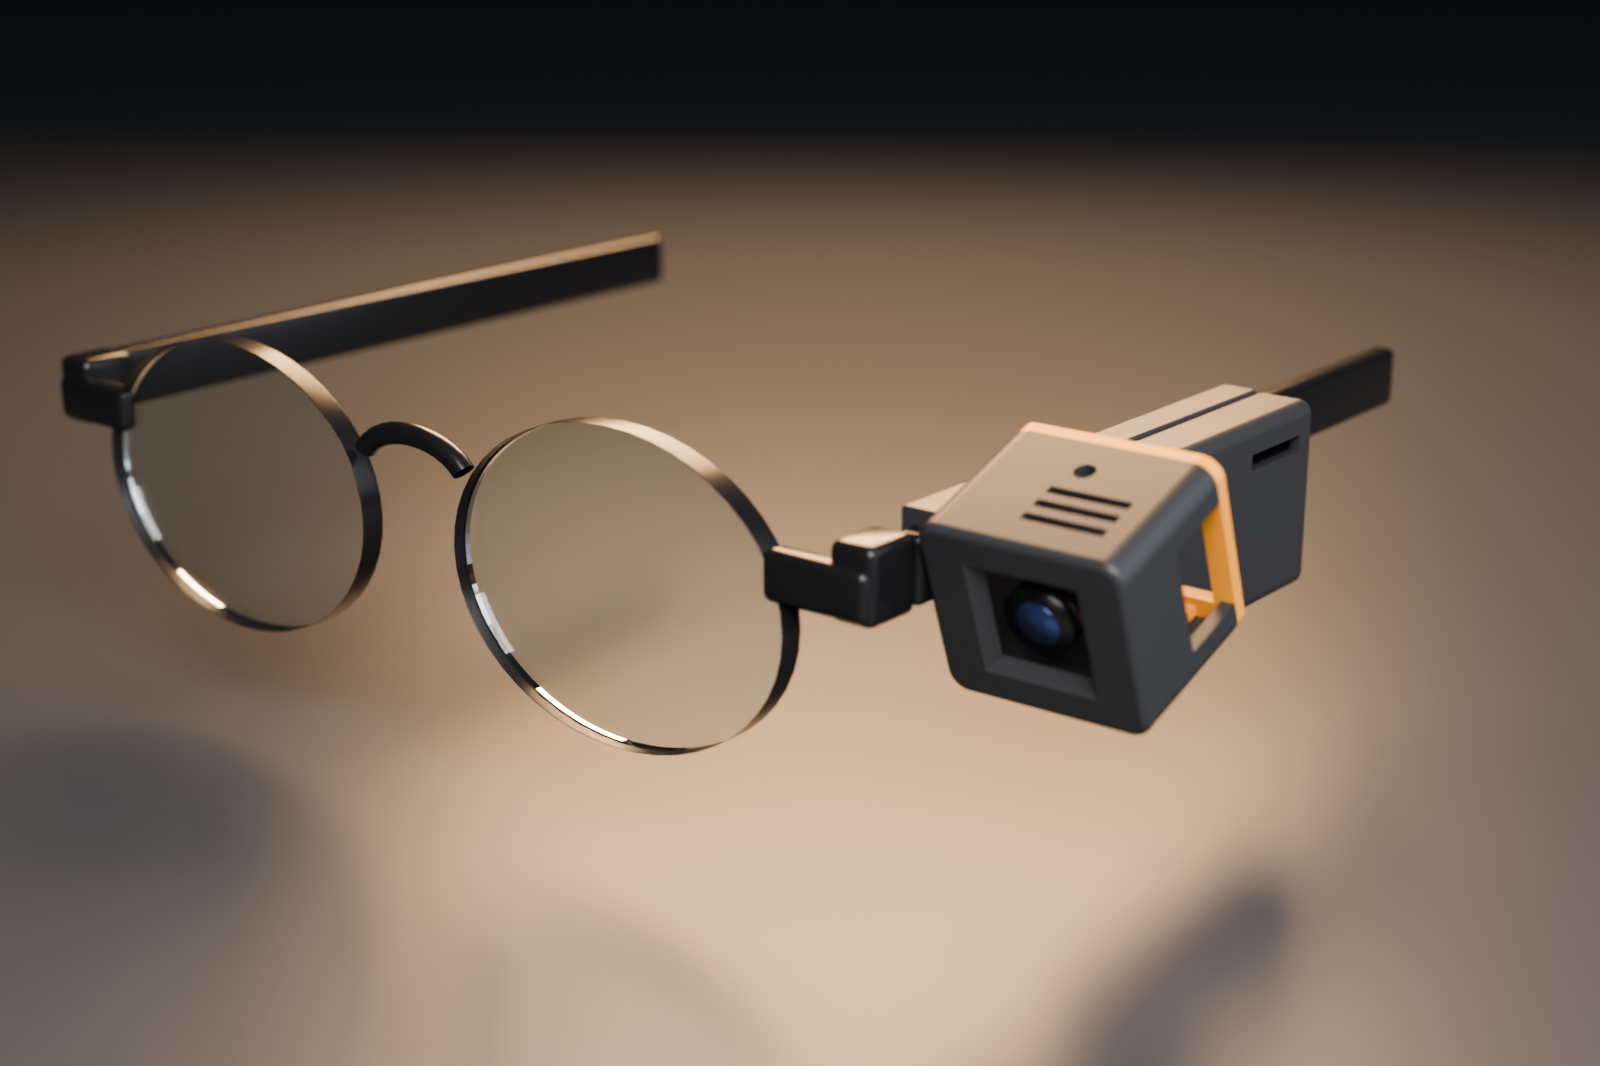
\includegraphics[width=\columnwidth]{figs/glasses_hero.png}
\caption{Camera glasses: printed camera pod (XIAO ESP32S3 Sense behind a
square window, tilted \SI{20}{\degree} down) and battery pod clipped to the
right temple arm of an ordinary frame. Rendered from the printable CAD files;
the frame is a generic stand-in.}
\label{fig:glasses}
\end{figure}
The capture device is a clip-on camera for an ordinary spectacle frame
(Fig.~\ref{fig:glasses}). A Seeed XIAO ESP32S3 Sense (OV2640, 8\,MB PSRAM,
$21\times17.8$\,mm) sits in a printed pod that hooks over the temple arm; a
single-cell 3.7\,V LiPo sits in a second pod behind it and is charged through
the board's own USB-C port, so there is no separate charger board. The only
wiring is the two battery leads and an optional push button on D1; the
board's BOOT button works as the trigger without it. The two pods weigh about
4.6\,g and 5.5\,g of solid PLA by CAD volume and print without supports. The
CAD is parametric, so a different temple-arm thickness or height means
editing two numbers and re-exporting the STL files.

One press records a burst of 13 JPEG frames at $1600\times1200$, 350\,ms
apart, into PSRAM while the wearer turns their head slowly across the plate,
about 4\,s in total. The firmware exposes \texttt{/status}, \texttt{/trigger},
\texttt{/frame?i=}, \texttt{/capture} and \texttt{/camera}; the host client
(\texttt{glasses\_client.py meal --phase served|cleared}) waits for the burst,
checks that every frame is a JPEG, and files it under the meal. It refuses a
\emph{cleared} burst for a meal with no \emph{served} burst, and a second
burst for the same phase. All reconstruction runs on the host. The firmware
compiles for the XIAO ESP32S3 target (Arduino core 3.3.12) and the client
passes tests against a simulated device; the glasses have not yet been
printed, flashed or worn, so no physical number is reported for them.
